\documentclass[11pt]{article}
\usepackage[margin=1in]{geometry}
\usepackage{graphicx,booktabs,amsmath,amssymb,xcolor,caption,subcaption}
\usepackage[hidelinks]{hyperref}
\usepackage{times}
\captionsetup{font=small,labelfont=bf}
\definecolor{slate}{HTML}{4A5D7E}
\definecolor{brick}{HTML}{8B3A3A}
\newcommand{\slate}[1]{\textcolor{slate}{#1}}

\title{\textbf{Two Kinds of Asynchrony:\\ Separating Concurrency from In-Flight Weight
Updates\\ in Asynchronous Reinforcement Learning}}
\author{Rajat Dandekar\\ \small Vizuara AI Labs\\
\small \texttt{pipelinerl-race.vercel.app}}
\date{\today}

\begin{document}
\maketitle

\begin{abstract}
\noindent
\emph{Synchronous} reinforcement learning on language models alternates between two workloads
that want opposite hardware: \emph{generation}, which is memory-bound and finishes at wildly
different times per sequence, and \emph{training}, which is compute-bound and synchronous.
Frameworks such as veRL run them in lockstep, so the cluster idles while it waits for the
slowest sequence in each batch.

\emph{Asynchronous} RL breaks that lockstep --- but it breaks it in two independent ways.
PipelineRL (Piché et al., 2025) both runs generation and training \emph{concurrently} on
disjoint GPUs, and pushes new weights into the running inference engine \emph{mid-sequence}
without discarding the KV cache, reporting ${\approx}2\times$ on 128 H100s. These are
different kinds of asynchrony: one \emph{spatial} --- different GPUs doing different things at
the same moment --- and one \emph{temporal} --- the policy changing while a sequence is still
being written. Every reported speedup bundles them, and no published measurement separates
them.

We therefore run three arms that share model, data, GRPO
implementation, batch shape, seed, library versions and total GPU budget, and differ only in
\emph{when each GPU does what}: (A) conventional alternation; (B) concurrent generation and
training with weights applied between generation batches; (C) concurrent with genuine
in-flight updates. On $2\times$H100 with Qwen2.5-1.5B on GSM8K, 45 minutes per arm, we find
that \textbf{concurrency alone doubles throughput} ($14.3 \to 29.4$ samples/s) and cuts idle
GPU-time $7.2\times$ ($1861 \to 258$ GPU-seconds), while \textbf{in-flight updates --- which
demonstrably work, 514/514 landing mid-decode with the cache retained --- buy nothing
measurable at this scale}, halving an already-negligible staleness ($0.051 \to 0.035$ steps)
at a ${\sim}7\%$ throughput cost. We also report a result we cannot yet attribute: both
concurrent arms end lower on reward, and the arms begin at different rewards \emph{before}
training can separate them, which we trace to a tensor-parallel difference in the generator
rather than to the scheduler. We release the harness, which enforces its own fairness
contract in code --- refusing to emit a figure when GPU-second accounting fails, when an arm
leaves a GPU idle, or when any arm's environment fingerprint differs.
\end{abstract}

\section{Introduction}

The RL loop for a language model is a systems problem before it is an algorithmic one. A
policy generates completions, a verifier scores them, and a trainer takes a gradient step.
The generation phase is memory-hungry and embarrassingly parallel; the training phase is
compute-hungry and synchronous. Running both on the same accelerators means one of them is
always waiting.

Conventional implementations accept this and alternate. veRL / HybridFlow~\cite{verl}
makes the alternation as cheap as possible --- resharding the actor between an
inference-optimal and a training-optimal layout with its 3D-HybridEngine, and searching for a
good device placement automatically --- and reports $1.5$--$20\times$ throughput over prior
systems. But the alternation itself remains: while any sequence in the batch is still
decoding, the GPUs that finished early have nothing to do.

PipelineRL~\cite{pipelinerl} attacks that residual idle time directly. Its two changes are:

\begin{enumerate}
\item \textbf{Concurrency.} Partition the cluster. Some GPUs generate forever; others train
forever. Neither waits for the other's phase.
\item \textbf{In-flight weight updates.} Because the generators never stop, their weights
would grow stale. So the trainer pushes new weights \emph{into a running engine}: generation
pauses between decode steps, the weights are swapped, the KV cache is retained, and sequences
already in progress continue under the new policy --- producing sequences whose early tokens
came from an older policy than their late tokens.
\end{enumerate}

These are logically independent. One could adopt concurrency alone and update weights at
batch boundaries; one could not sensibly do the reverse. The published comparison is
conventional versus \emph{both}, which leaves an obvious question unanswered: of the reported
speedup, how much is the partition and how much is the mid-sequence update?

\paragraph{Contributions.}
\begin{itemize}
\item A three-arm decomposition (\S\ref{sec:method}) isolating concurrency from in-flight
updates, with a fairness contract enforced mechanically rather than by convention.
\item A measurement (\S\ref{sec:results}) showing concurrency accounts for essentially the
entire throughput gain at small scale, and that in-flight updates are inert there --- with an
explanation of the regime in which they should matter.
\item A negative result and an honest attribution failure (\S\ref{sec:limits}): the
concurrent arms learn less per sample, but a generator-side confound prevents us from
attributing that to staleness.
\item An open-source harness (\S\ref{sec:harness}) whose validators refuse to publish
malformed comparisons --- built after several of our own runs produced confident, well-formed,
wrong numbers.
\end{itemize}

\section{Method}\label{sec:method}

\subsection{The three arms}

All arms optimise the same objective with the same code. We use GRPO~\cite{grpo}: for each
prompt, $G$ completions are sampled, the group's mean reward forms the baseline, and the
token-level clipped policy-gradient loss is applied with group-normalised advantages. The
reward is binary and verifiable --- $1$ if the final numeric answer matches GSM8K's gold
answer, else $0$ --- so there is no reward model and nothing to hack.

\begin{description}
\item[A --- Conventional.] All $N$ GPUs alternate. vLLM runs tensor-parallel across all of
them for generation; the engine then sleeps, releasing its KV cache so the trainer can use
the memory; the trainer steps; weights are pushed back and the engine wakes. Data is always
perfectly on-policy ($\mathrm{lag}=0$ by construction). This is the colocated HybridEngine
pattern, and the PipelineRL authors note that veRL's throughput should resemble their
conventional baseline.
\item[B --- Concurrent, batch-boundary updates.] The GPUs are partitioned once: $k$ generate
continuously, $N-k$ train continuously. A producer keeps the inference engine saturated; a
consumer trains on completed rollouts. Weights are applied \emph{between} generation batches.
\item[C --- Concurrent, in-flight updates.] Identical partition, but the update is issued
against a running engine via \texttt{pause\_generation(mode="keep",\ clear\_cache=False)},
\texttt{collective\_rpc\_async}, \texttt{resume\_generation}. The engine halts between decode
steps, in-flight requests and their KV blocks survive, and decoding resumes under the new
weights.
\end{description}

\subsection{The fairness contract}

A three-way comparison is worth nothing unless the arms differ in exactly one respect. We
enforce this in code rather than by discipline:

\begin{itemize}
\item \textbf{One} GRPO implementation and \textbf{one} batching path, imported by all arms.
No arm has its own loss.
\item A \texttt{fairness\_key()} covering every hyper-parameter \emph{and an environment
fingerprint} (vLLM / PyTorch / Transformers versions, GPU model), compared after the run. A
mismatch aborts publication. This is not hypothetical: the in-flight arm requires
vLLM $\geq$ 0.18, and an earlier iteration of this study ran arms on 0.11 and 0.18, which
would have confounded ``scheduling'' with ``inference engine upgraded''.
\item A \textbf{placement check}: each arm verifies at start-up that its trainer is not on an
inference GPU and that every inference GPU actually holds an engine.
\item A \textbf{GPU-second invariant}: every GPU is in exactly one state at every instant, so
accounted GPU-seconds must equal $N \times$ duration. Violation means the event stream is
out of order, and the analyser refuses to report a utilisation split rather than reporting a
plausible one.
\item An \textbf{unused-GPU check}: an arm that leaves a GPU idle raced with a handicap. Our
first four-GPU attempt did exactly this --- the trainer was single-GPU while the partition
allocated two --- and the resulting ``conventional wins'' was an artefact of the missing GPU.
\end{itemize}

The only quantity an arm may interpret differently is how the fixed GPU budget is
\emph{partitioned}.

\subsection{Telemetry}

Every GPU state transition, weight transfer, and finished rollout appends one line to a
single JSONL stream. All figures and all reported numbers derive from that one stream, so a
plot and an animation of the same run cannot disagree. Idle is emitted explicitly and
eagerly; a stream that omitted idleness would make the arms look identical. Timestamps are
taken under the writer's lock --- sampling them outside it allowed two threads to stamp
out-of-order lines, which inflated integrated GPU-seconds beyond the cluster's capacity and
was caught only by the invariant above.

\section{Experimental setup}

Qwen2.5-1.5B-Instruct on GSM8K, $2\times$H100, 45 minutes of wall-clock per arm after engine
start-up (reported separately). $G=8$ completions per prompt, 16 prompts per optimizer step
(128 samples/step), up to 512 new tokens, temperature $1.0$, learning rate $10^{-6}$,
clipping $\varepsilon=0.2$, no KL penalty. Arms B and C use one generation GPU and one
training GPU; arm A time-shares both.

Two GPUs rather than four is a deliberate consequence of the fairness contract. Our trainer
is single-GPU, so a fair split needs $k = N-1$ generation GPUs; at $N=4$ that requires
$\mathrm{TP}=3$, which vLLM cannot shard for a model with 2 key--value heads. Two GPUs is
therefore the largest configuration in which no GPU is stranded. We regard this as a real
limitation of the study, not a detail (\S\ref{sec:limits}).

Weight transfer uses CUDA IPC handles: \texttt{reduce\_tensor} yields a picklable handle the
inference workers reopen against the sender's GPU memory, so nothing crosses PCIe. The
transport is chosen \emph{before} the first push from
\texttt{torch.cuda.can\_device\_access\_peer}, never by catching an exception --- an exception
inside \texttt{collective\_rpc} poisons the vLLM executor, so a runtime fallback would kill
the engine on first use.

\section{Results}\label{sec:results}

\begin{table}[h]
\centering
\small
\begin{tabular}{lrrr}
\toprule
 & \textbf{A} conventional & \textbf{B} concurrent & \textbf{C} concurrent+in-flight \\
\midrule
samples generated            & 38{,}784 & 80{,}256 & 74{,}112 \\
samples / second             & 14.34 & \textbf{29.37} & 27.39 \\
\quad vs.\ conventional      & --- & \textbf{2.05$\times$} & 1.91$\times$ \\
GPU-seconds idle             & 1861.1 & 1638.4 & \textbf{257.7} \\
GPUs computing (mean)        & 65.6\% & 70.0\% & \textbf{95.2\%} \\
optimizer steps              & 303 & 562 & 514 \\
weight updates               & 303 & 562 & 514 \\
\quad of which in-flight     & 0 & 0 & \textbf{514} \\
mean weight-push (ms)        & 453.3 & 319.9 & 260.5 \\
mean lag (optimizer steps)   & 0.0 & 0.051 & 0.035 \\
reward, final 10\% of samples & 0.7476 & 0.6888 & 0.6826 \\
reward at matched samples    & 0.7476 & 0.6978 & 0.6929 \\
\bottomrule
\end{tabular}
\caption{All three arms, identical budget and hyper-parameters, 45 minutes each. The
fairness key --- including library versions --- matched exactly across arms.}
\label{tab:main}
\end{table}

\subsection{Concurrency doubles throughput}

Arm B generates $2.05\times$ the samples per second of arm A. Figure~\ref{fig:util} shows the
mechanism directly: the fraction of GPUs actually computing, over time. Arm A sags on every
generate/train alternation and averages 64\%; arm C is a near-solid block at 95\%. The
white space above each curve is compute that was paid for and not used, and it falls
$7.2\times$ from arm A to arm C.

\begin{figure}[h]
\centering
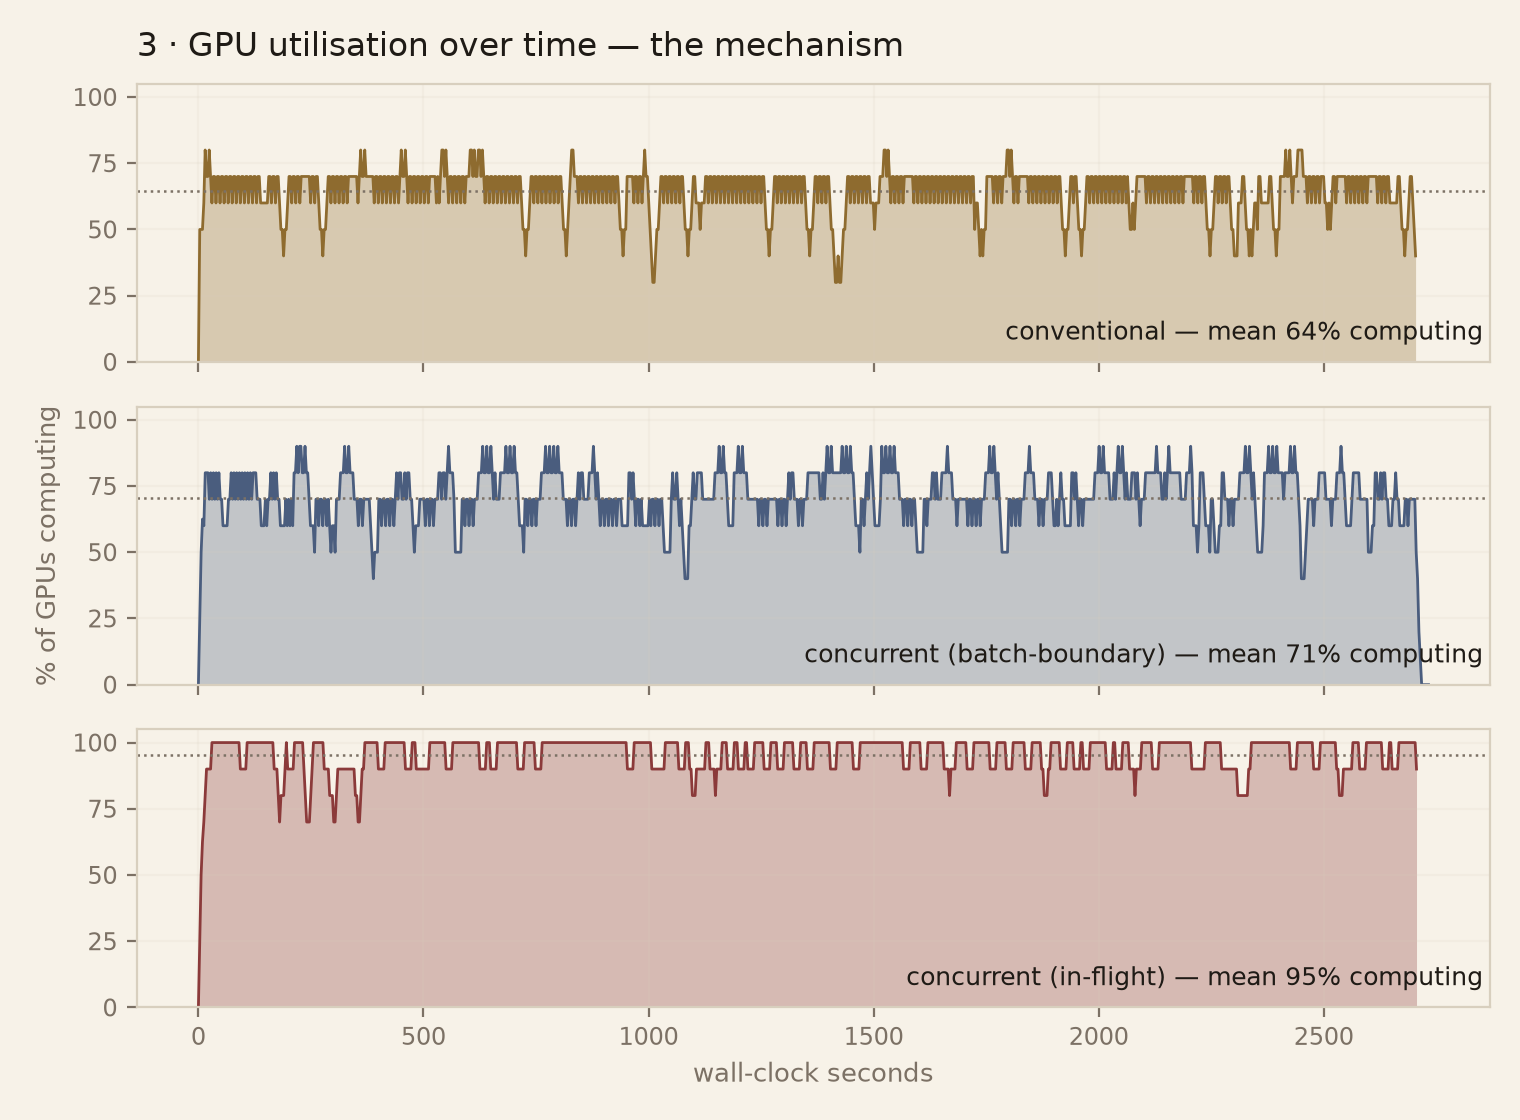
\includegraphics[width=0.68\textwidth]{figs/g3_gpu_utilisation.png}
\caption{GPU utilisation over time. The alternation bubble is visible in arm A as periodic
sags; the in-flight arm removes it almost entirely.}
\label{fig:util}
\end{figure}

\subsection{In-flight updates work --- and are inert at this scale}

All 514 of arm C's weight updates landed mid-decode with the KV cache retained; we verified
separately on a live engine that the KV block count is unchanged across a pause--update--resume
cycle while a 384-token generation is in flight, and that the request still completes. The
mechanism is real.

Its effect is not. Arm C halves mean lag relative to arm B ($0.051 \to 0.035$ optimizer
steps) and costs ${\sim}7\%$ throughput, and Figure~\ref{fig:reward}(right) shows the two
concurrent arms' learning curves lying on top of one another. The explanation is simply that
at two GPUs there is almost no staleness to remove: 95\% of arm B's samples are \emph{already}
perfectly on-policy, because a generation batch completes in roughly the time of one optimizer
step. In-flight updates are a solution to a problem that does not exist at this scale.

We would expect them to matter when lag is large --- many generation GPUs per trainer, long
sequences, high length variance --- which is precisely the 128-GPU regime the original paper
measures.

\begin{figure}[h]
\centering
\begin{subfigure}{0.49\textwidth}
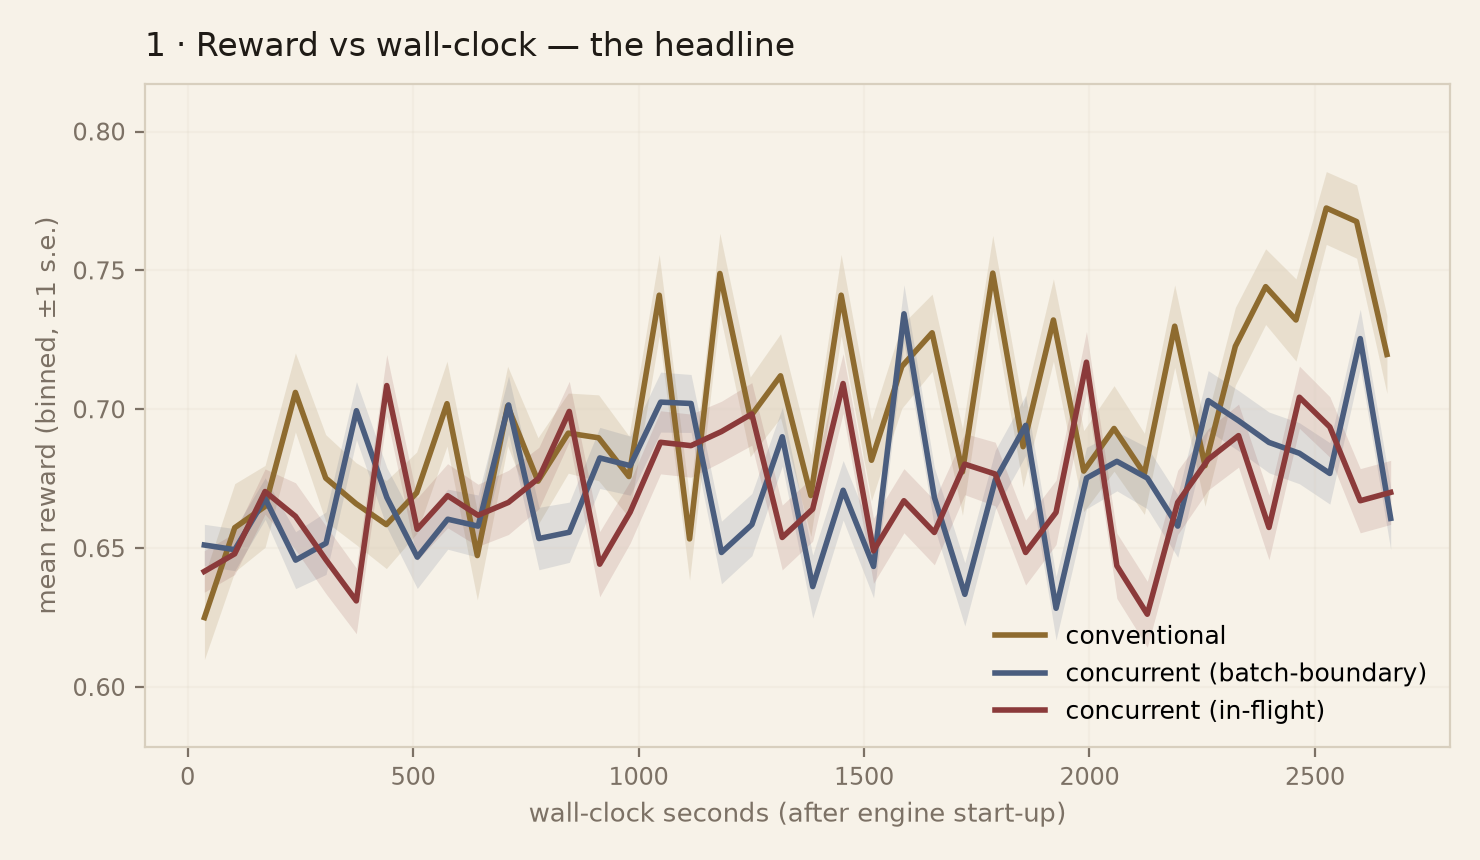
\includegraphics[width=\textwidth]{figs/g1_reward_vs_wallclock.png}
\end{subfigure}
\begin{subfigure}{0.49\textwidth}
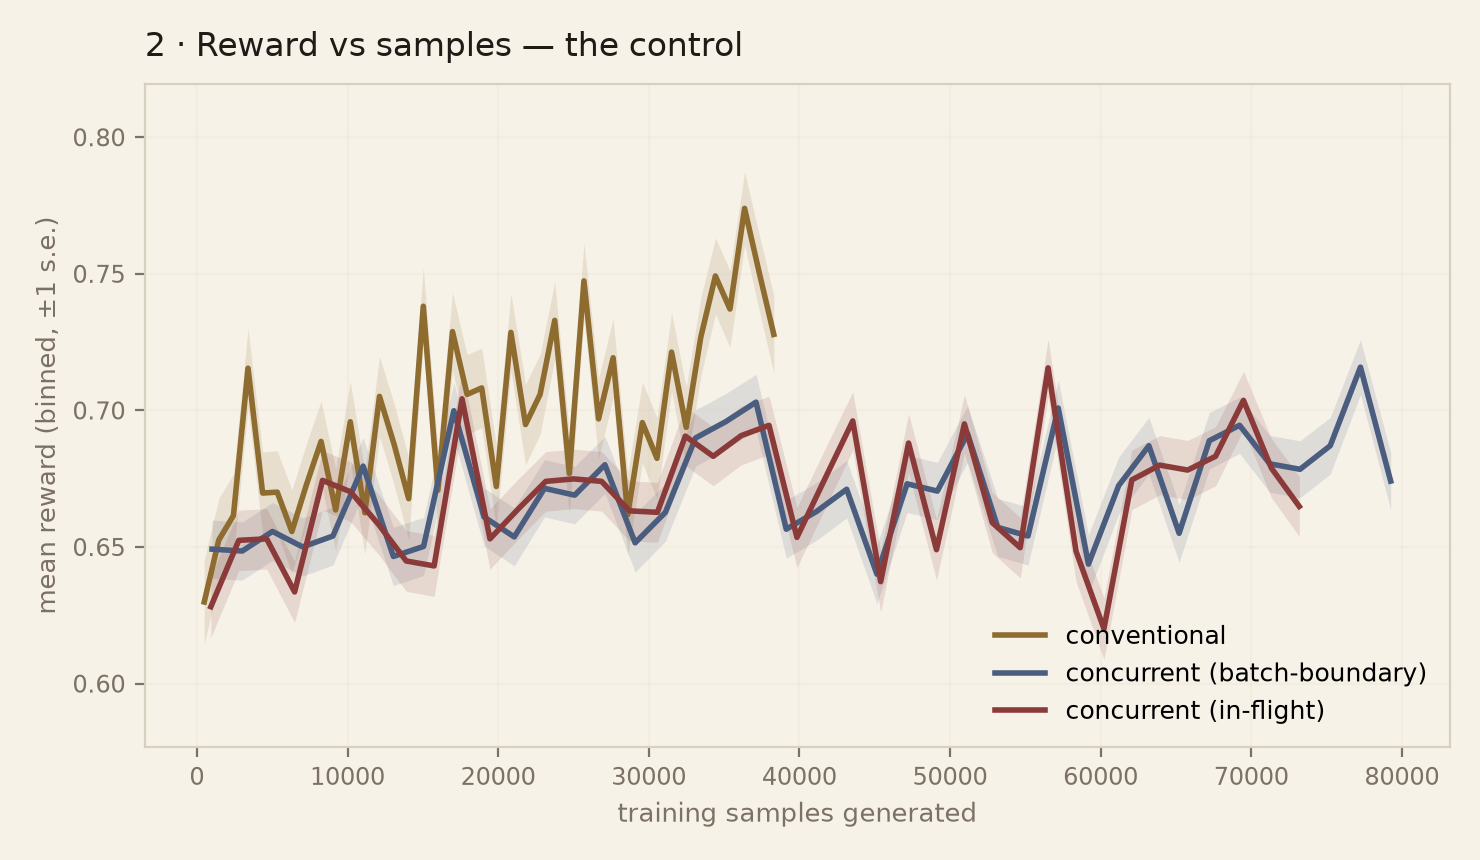
\includegraphics[width=\textwidth]{figs/g2_reward_vs_samples.png}
\end{subfigure}
\caption{Reward against wall-clock (left) and against samples generated (right). The two
concurrent arms coincide, indicating in-flight updates changed learning by nothing
measurable. Both sit below conventional --- see \S\ref{sec:limits} for why we do not
attribute that to the scheduler.}
\label{fig:reward}
\end{figure}

\subsection{Small staleness, visible in the loss}

Although lag is small, it is not invisible. Figure~\ref{fig:stale} shows that the fraction of
tokens whose importance ratio leaves the trust region climbs from ${\approx}0.12\%$ to
${\approx}0.35\%$ over training for both concurrent arms, while the conventional arm stays
flat. As the policy moves faster, the same one-step lag displaces the ratio further. This is
the mechanism by which staleness would eventually cost effectiveness --- observable here, but
far too small to explain the reward gap in Table~\ref{tab:main}.

\begin{figure}[h]
\centering
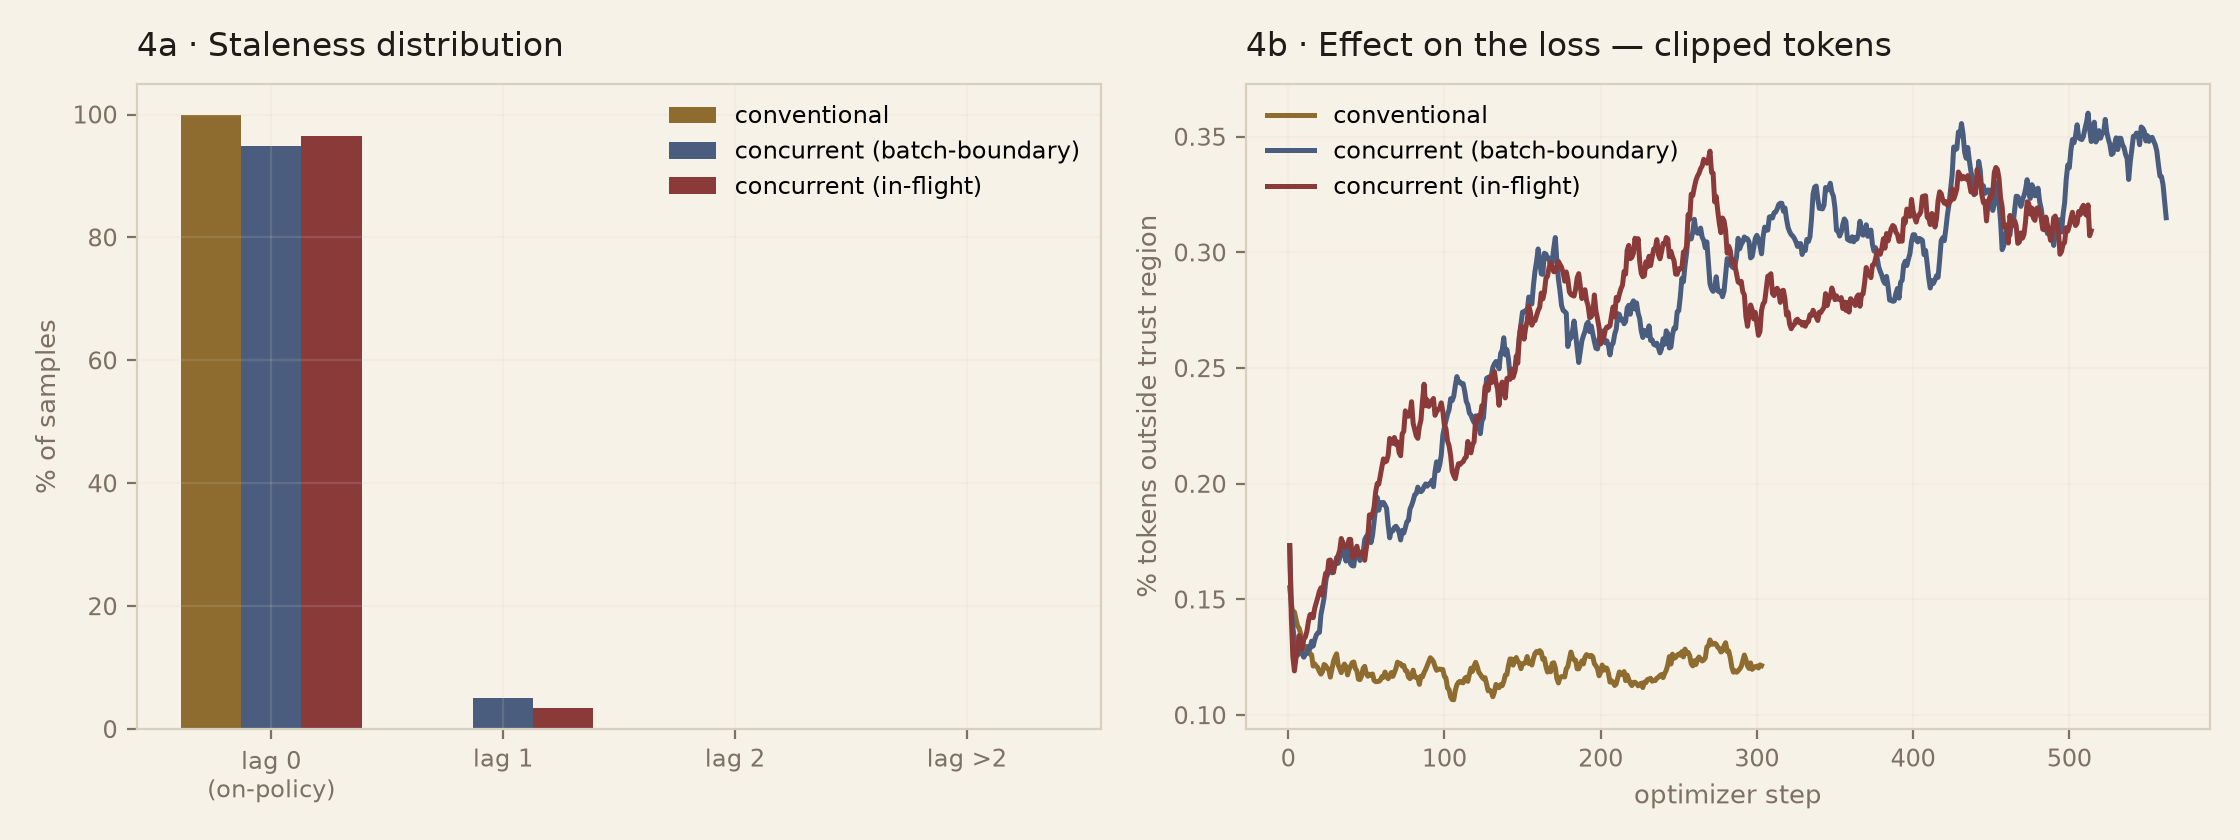
\includegraphics[width=0.92\textwidth]{figs/g4_staleness.png}
\caption{Left: distribution of per-sample lag. Right: clipped-token fraction over training,
the effect of that lag on the loss.}
\label{fig:stale}
\end{figure}

\section{Limitations and an unattributed result}\label{sec:limits}

\paragraph{The concurrent arms learn less per sample, and we cannot say why.}
At matched sample budget --- identical prompts in identical order --- arm A reaches $0.7476$
against $0.6978$ and $0.6929$. That is a real difference, but we decline to attribute it to
staleness, because the arms \emph{begin} at different rewards: over their first 10\% of
samples, $0.6650$, $0.6510$ and $0.6417$ respectively, before training could have separated
them. Same base model, same seed, same prompts.

The likely cause is the generator, not the scheduler. Arm A generates with $\mathrm{TP}=2$
and arms B and C with $\mathrm{TP}=1$; tensor-parallel reduction order changes logits at the
last bit, and under temperature-1 sampling a perturbed logit changes the entire sampled
trajectory. The arms are therefore drawing from measurably different sampling distributions
before any learning occurs. Settling this requires (i) evaluating on a held-out set with
fixed decoding rather than reading reward off training rollouts, and (ii) matching generator
tensor-parallelism across arms, e.g.\ by running data-parallel $\mathrm{TP}=1$ engines in the
conventional arm. We regard the throughput and utilisation results as sound and the learning
comparison as open.

\paragraph{Scale.} Two GPUs compresses the effect under study. The idle bubble grows with
cluster size and with sequence-length variance; a two-GPU cluster has one generation GPU, so
there is no ``other GPUs wait for the straggler'' effect at all --- only the phase alternation.
Our headline is therefore a lower bound on what concurrency buys.

\paragraph{Staleness measurement.} Lag is recorded when a sequence \emph{completes}, which is
a lower bound: a sequence spanning an in-flight update has tokens of several policy ages, and
we record only the count of versions that landed while it decoded. Reporting per-token
effective sample size would be stricter; our harness now logs the necessary statistic, but
the runs reported here predate it and we do not substitute a proxy silently.

\paragraph{Single seed.} Each arm was run once. The throughput and utilisation differences are
far outside plausible run-to-run variation; the reward differences are not obviously so.

\section{The harness}\label{sec:harness}

Building this taught us more than the result did. Six distinct bugs in our own code produced
\emph{confident, well-formed, wrong} output rather than crashing: telemetry timestamps taken
outside the writer's lock; a vLLM executor that returns a stale error to every subsequent call
after one failure, making a healthy component report as broken; a
\texttt{CUDA\_VISIBLE\_DEVICES} leak that silently co-located the trainer with the generator
while still reporting a clean split; an optimizer-offload ordering error; a utilisation metric
counting \texttt{waiting} as busy, which reported 97.8\% for an arm with a completely idle
GPU; and a GRPO grouping error in which one rollout per prompt made the advantage baseline
average over unrelated questions.

Every one of these is now an assertion that refuses to proceed, and the assertions are the
part of this artifact we would most encourage others to copy. A comparison harness that
cannot fail loudly will eventually publish something false.

\section{Related work}

veRL / HybridFlow~\cite{verl} formalises RLHF as a hybrid-controller dataflow and makes the
colocated alternation efficient. PipelineRL~\cite{pipelinerl} introduces concurrent
generation/training with in-flight weight updates. GRPO~\cite{grpo} removes the critic by
using a group baseline. Our contribution is not a new method but a decomposition and an
honest measurement of an existing one at small scale, plus the validation harness that makes
such measurements trustworthy.

\begin{thebibliography}{9}
\bibitem{verl} G. Sheng, C. Zhang, Z. Ye, X. Wu, W. Zhang, R. Zhang, Y. Peng, H. Lin, C. Wu.
\emph{HybridFlow: A Flexible and Efficient RLHF Framework}. arXiv:2409.19256, 2024.
\bibitem{pipelinerl} A. Piché et al. \emph{PipelineRL: Faster On-policy Reinforcement Learning
for Long Sequence Generation}. arXiv:2509.19128, 2025.
\bibitem{grpo} Z. Shao et al. \emph{DeepSeekMath: Pushing the Limits of Mathematical Reasoning
in Open Language Models}. arXiv:2402.03300, 2024.
\bibitem{gsm8k} K. Cobbe et al. \emph{Training Verifiers to Solve Math Word Problems}.
arXiv:2110.14168, 2021.
\end{thebibliography}

\end{document}
